\chapter{Entwicklung der Modellierungssprache}
\label{ch:Implementation}
Bevor die ausgearbeiteten Konzepte in das \emph{TherapyBuilder}-Projekt eingearbeitet werden, werden diese zunächst in einem Prototypen umgesetzt. Da bereits das Experience Sampling Tool \emph{movisensXS} existiert, welches Studien, die Chatbot-ähnliche Dialoge beinhalten, umsetzen kann, wird dieses an die ausgearbeiteten Anforderungen angepasst. Auf diese Weise soll später eine Studie durchgeführt werden, die das Konstruktionsprinzip und die Sprünge mit den Ansätzen des dort verwendeten Konfigurationsprinzips und Sichtbarkeitsregeln vergleicht. Das Konfigurationsprinzip geht mit Einschränkungen in der Flexibilität einher die das Konstruktionsprinzip, dank des Baukastenprinzips, anbietet. Auch ist nicht klar, ob spätere Nutzer die Metapher der Sprünge nachvollziehen können. Verglichen werden diese mit den Sichtbarkeitsregeln des \emph{movisensXS}-Systems. Diese Regeln agieren als eine Art Filter, die regulieren, wann ein Element für eine Nutzergruppe sichtbar wird. 

Die ausgearbeiteten Konzepte werden für die Studie als \emph{TherapyBuilder} Klick-Prototyp umgesetzt. Für den direkten Vergleich mit dem \emph{movisensXS}-System, wird dieses an die Anforderungen angepasst. Hierfür wird eine Bibliothek geschrieben, die entsprechende Elemente der Anforderungsliste, die im Handelsüblichen fehlen, hinzufügt, anpasst und andere Elemente entfernt. Im Folgenden wird die Umsetzung der Prototypen beschrieben.


\section{TherapyBuilder-Prototyp}
Wie zuvor beschrieben werden die Ausgearbeiteten Konzepte des Konfigurationsprinzips und Sprünge für die spätere Evaluation in einem Klick-Prototyp umgesetzt. Die Web App \emph{moqups}(vgl. \cite{OnlineMo52:online}) besitzt die Möglichkeit aufwändige Klick-Protoptypen umzusetzen. Dieses Tool wurde für den Bau des Prototyps verwendet. Dem Studienteilnehmer soll später den Eindruck eines funktionierenden Programms vermittelt werden. Hierfür werden im Klick-Prototyp alle möglichen Funktionen abgebildet. Dies beginnt bereits mit einer Eingangsseite, die eine Übersicht aller bisher angelegten Therapie-Module bietet. Zunächst wird auf dieser exemplarisch ein Therapie-Modul angeboten. Abbildung \ref{start} zeigt die Ansicht der Eingangsseite, die dem Probanden präsentiert wird. 

\begin{figure}[h]
\centering
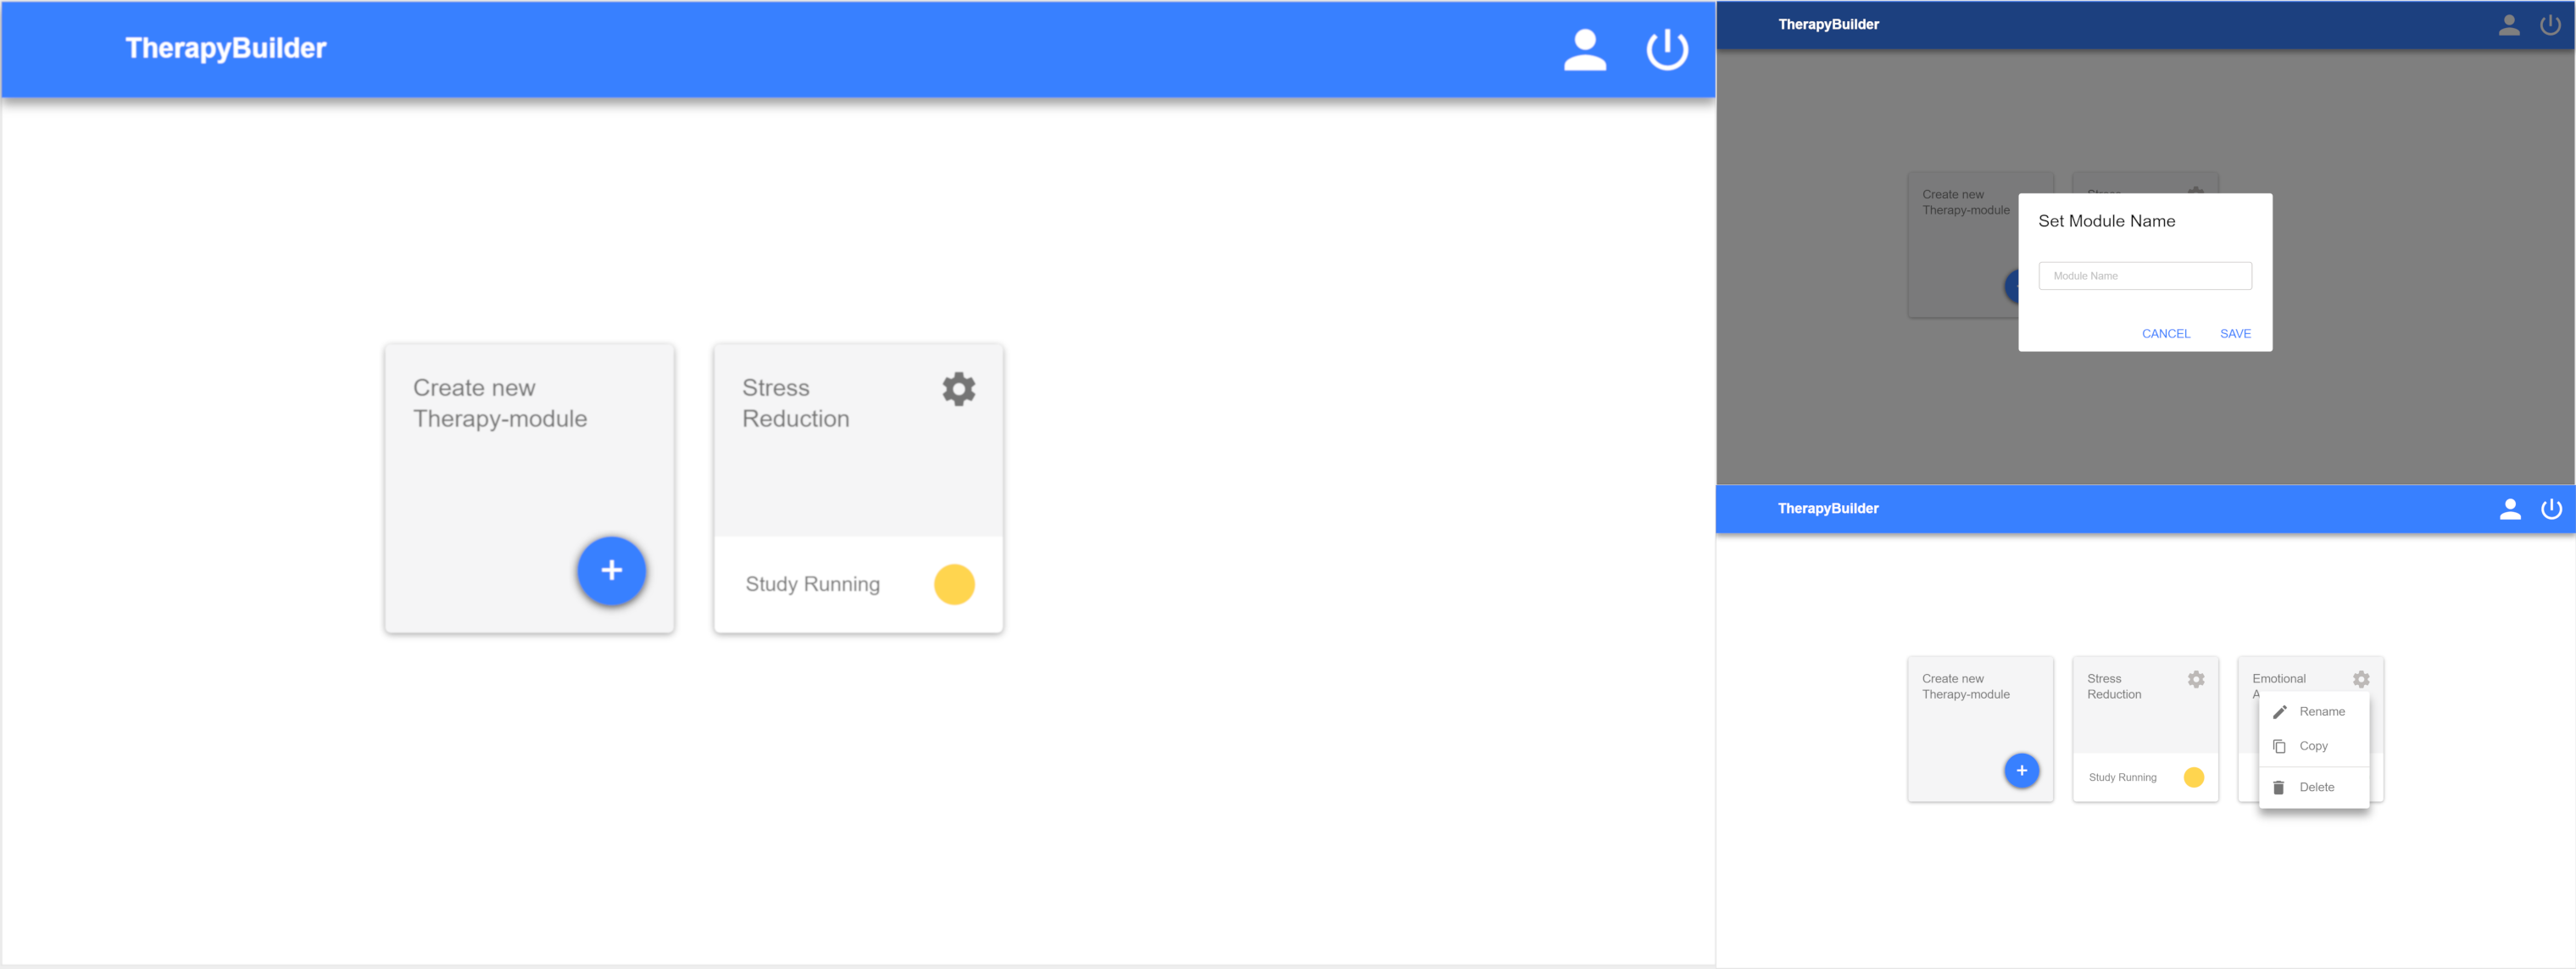
\includegraphics[width=1\textwidth]{pictures/start}
\caption{Die Eingangsseite des \emph{TherapyBuilder}-Prototyps. Diese vermittelt dem Studienteilnehmer den Eindruck ein funktionsfähiges Programm zu betrachten.}
\label{start}
\end{figure}

Der Proband hat die Möglichkeit einzelne Elemente anzuklicken um spätere mögliche Funktionen zu entdecken. Diese beinhalten die Möglichkeit ein neues Therapie-Modul anzulegen. Ein Klick auf den entsprechenden Button öffnet einen Overlay zur Namensvergabe und speichern des Moduls. Auch Einstellungsmöglichkeiten können, durch Klick des Zahnrades, angezeigt werden. Klickt der Proband auf das bereits angelegte Modul \emph{Stress Reduction}, so gelangt dieser auf die zeitliche Darstellung des Therapie-Moduls. Dieses setzt das, in Kapitel \ref{ch:design} beschriebene Konfigurationsprinzip um. Dieses wird nachfolgend dargestellt. Abschließend wird die Umsetzung der Sprünge präsentiert.

\subsection{Konfigurationsprinzip}
Wurde ein Therapie-Modul angeklick, öffnet sich die zeitliche Darstellung der Konfigurationen. Damit die Probanden einen Eindruck erhalten, wie ein Therapie-Modul in dieser Darstellungsform aussehen wird, wurde eine Vielzahl von Konversationen angelegt, deren Trigger bereits eingestellt wurden. Die Konversationen unterscheiden sich in Farbe, Dauer, Icons und Frequenz. 
 
\begin{figure}[h]
\centering
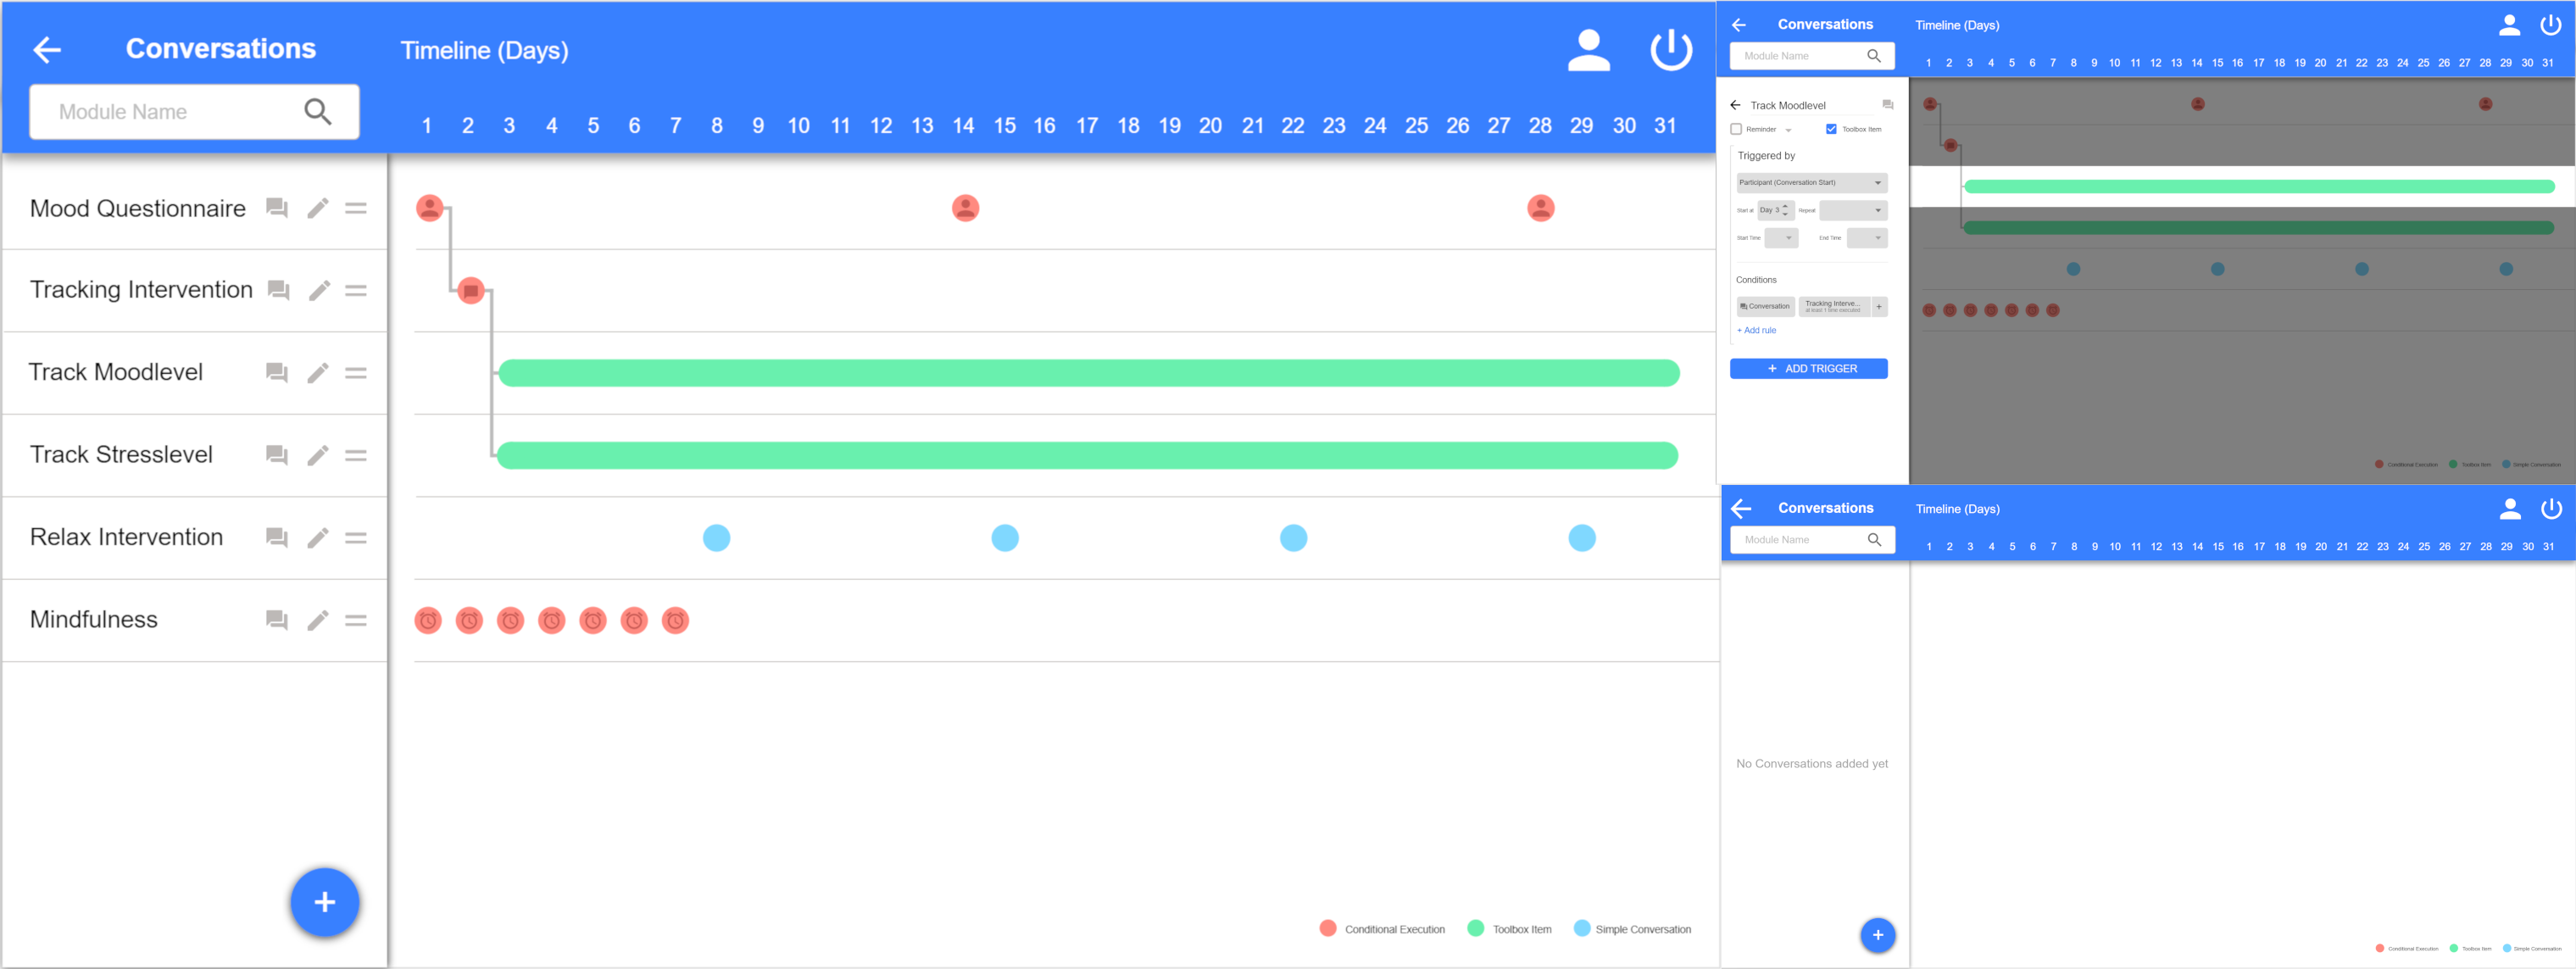
\includegraphics[width=1\textwidth]{pictures/zeitstrahl}
\caption{Das Konfigurationsprinzip beinhaltet eine zeitliche Darstellung aller Chatbot-Konversationen.}
\label{zeitstrahl}
\end{figure}

Der Proband hat die Möglichkeit die Trigger-Einstellungen jeder Konversation aufzurufen. Auch kann der Proband verschiedene Einstellungsmöglichkeiten erkunden. Allerdings kann er in dieser Ansicht keine Einstellungen vornehmen. Dies ist in einer anderen, vorbereiteten Ansicht möglich. Hat der Proband auf der Startseite das Therapie-Modul \emph{Emotional Awareness} erzeugt und ruft dessen zeitliche Darstellung auf, so erhält er in dieser zunächst ein leeres Arbeitsblatt. Dort hat er die Möglichkeit eine Konversation zu erstellen und in dieser, eingeschränkt, Trigger-Einstellungen vorzunehmen. Einstellen kann er dabei nur die Werte, die in den Aufgaben der Studie vorgegeben werden. Klickt der Proband auf das Dialog-Icon einer Konversation, so öffnet sich die nächste Ansicht. In dieser wird die Chatbot-Konversation dargestellt. 

\subsection{Sprünge}
Wurde die Chatbot-Konversation des Therapie-Moduls \emph{Stress reduction} aufgerufen, wird eine bereits angelegte Darstellung geöffnet, die keine Einstellungsmöglichkeiten bietet und nur zum erkunden dient. Wurde die Chatbot-Konversation des Therapie-Moduls \emph{Emotional awareness} geöffnet, kann der Proband eingeschränkt eine Chatbot-Konversation anlegen. Die Chatbot-Konversation kann sehr bedingt eingestellt werden. Die Einstellungsmöglichkeiten werden auch hier von der Aufgabe der Studie vorgegeben. Die Ansicht der Chatbot-Konversation des Therapie-Moduls \emph{Stress Reduction} besteht aus einer Liste der Items, die zuvor im Kapitel \ref{ch:Design} beschrieben wurde. 

Die Ausgaben des Chatbots werden in einer grauen Sprechblase abgebildet. Die Sprechblase ist nach links orientiert ausgerichtet. Die Eingabeformate des Anwenders werden in einer blauen Sprechblase dargestellt. Der Proband hat hier die Möglichkeit auf verschiedene Nachrichten innerhalb der \emph{Lanes} zu klicken und die exemplarische Ansicht der Einstellung eines Elements zu öffnen. Diese sind nach rechts orientiert. Der Gesprächsverlauf wird in sogenannten \emph{Lanes} dargestellt. Zunächst wird dieser innerhalb einer \emph{Lane} angelegt. Wird ein alternativer Gesprächsverlauf dargeboten, so wird dies durch eine Condition, in Form eines runden Elements, angedeutet. Dieses runde Element kann entsprechend der Bedingung eingestellt werden und bestimmt, in welcher \emph{Lane} der alternative Gesprächsverlauf weitergeführt wird. 


\begin{figure}[h]
\centering
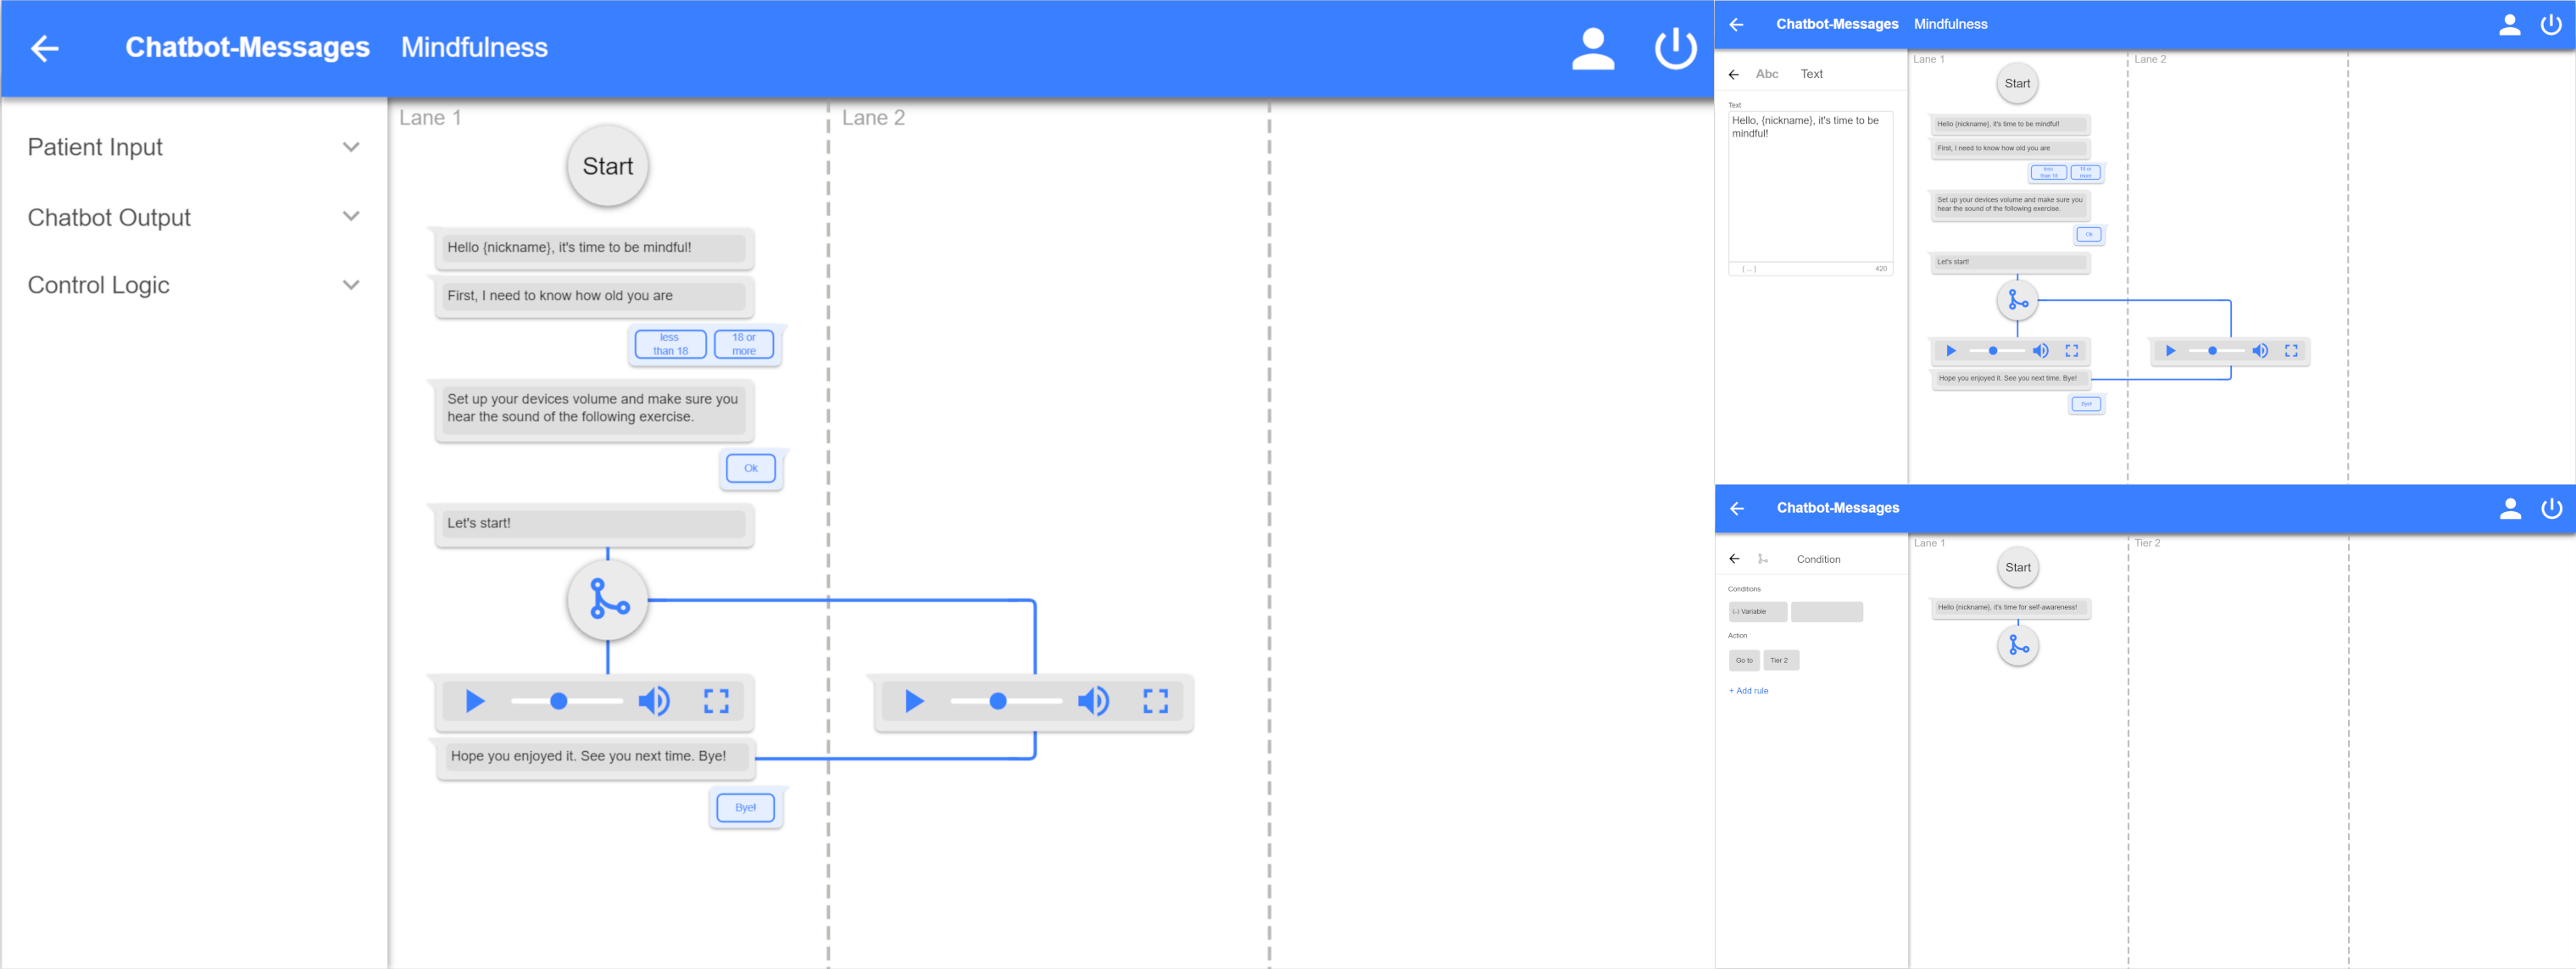
\includegraphics[width=1\textwidth]{pictures/textset}
\caption{Die Darstellung der Nachrichten. Der Proband hat die Möglichkeit verschiedene Nachrichten anzuklicken und die entsprechende exemplarische Einstellung zu öffnen. Die Ein Sprung im Konversationsverlauf wird durch ein Rundes Element dargestellt, welches auf verschiedene \emph{Lanes} verweist. Dieses Element kann im Therapie-Modul \emph{Emotional Awareness}exemplarisch konfiguriert werden.} 
\label{textset}
\end{figure}

\section{movisensXS-Prototyp}
Der \emph{movisensXS}-Prototyp besteht aus dem Hanndelsüblichen \emph{movisensXS}, welches lediglich eine angepasste Bibliothek verwendet, um die gelisteten Anforderungen aus Kapitel \ref{ch:Design} umzusetzen. In diesem Prototyp hat der Proband somit die Möglichkeit alle Funktionen zu erkunden. Gestartet wird dieser Prototyp lokal auf einem Rechner. Auch hier gibt es bereits das Therapie-Modul \emph{Stress reduction}. Dieses beinhaltet die gleichen Konversationen und Trigger-Einstellungen wie sie im \emph{TherapyBuilder}-Prototyp zu finden sind. Das \emph{movisensXS} beginnt ebenfalls mit einer Eingangsseite, die eine Übersicht der angelegten Therapie-Module bietet. 

\begin{figure}[h]
\centering
\includegraphics[width=1\textwidth]{pictures/movstart}
\caption{Die Eingangsseite des \emph{movisensXS}-Prototyps. Hier finden sich ebenfalls die Therapie-Module \emph{Emotional Awareness} und \emph{Stress Reduction}.}
\label{start}
\end{figure}

Klickt der Proband auf ein Modul, so wird dieser zunächst auf ein Dashboard weitergeleitet. Ausgehend von diesem kann die Ansicht der Trigger-Einstellungen oder die Liste aller Konversationen angezeigt werden. Die Trigger-Einstellungen implementieren das Konstruktionsprinzip.

\subsection{Konstruktionsprinzip}
Werden die Trigger-Einstellungen des \emph{Stress Reduction} aufgerufen, wird der Triggerbaum dargestellt. Dieser setzt sich aus folgenden Baukästen zusammen: \emph{Trigger}, \emph{Conditions} und \emph{Conversations}. \emph{Trigger} und \emph{Conditions} steuern wann und anhand welcher Bedingungen eine Konversation gestartet wird.  \emph{Conversations} lassen den Nutzer die Einstellung vornehmen, welche Konversation gestartet wird. Diese werden im Reiter \emph{Conversations} aufgerufen. 

Die Bausteine folgen dem Ampelprinzip. \emph{Trigger} werden mit der Farbe Rot, \emph{Conditions} mit der Farbe Gelb und \emph{Conversations} mit der Farbe Grün markiert. Diese farbliche Kodierung deutet an, zu welcher Zeit (\emph{Trigger}), zu welchen Bedingungen (\emph{Conditions}) die Konversation gestartet wird. Diese setzt auch die Reihenfolge der Verschaltung fest. Auf einen roten Baustein kann somit immer nur ein roter oder gelber Baustein folgen. Auf einen gelben Baustein kann immer nur ein grüner folgen. Dies wird zusätzlich durch die Form der Ecken der Bausteine verdeutlicht. Legt der Proband das \emph{Stress Reduction} Therapie-Modul an, kann dieser Trigger-Einstellungen für eine angelegte Konversation in Form eines Baumes anlegen.  

\begin{figure}[h]
\centering
\includegraphics[width=1\textwidth]{pictures/movtrig}
\caption{Die Trigger-Einstellungen des Therapie-Moduls \emph{Stress Reduction}. Links befindet sich die Werkzeugpalette mit den entsprechenden Bausteinen. Diese können per Drag and Drop auf dem Arbeitsblatt platziert werden. Einzelne Elemente werden}
\label{start}
\end{figure}



\subsection{Sichtbarkeitsregeln}
Damit eine Konversation innerhalb des Trigger-Baumes ausgewählt werden kann, muss diese zunächst im Reiter \emph{Conversations} angelegt werden. Auch hier befinden sich im Therapie-Modul \emph{Stress Reduction} die gleichen Inhalte wie im \emph{TherapyBuilder}-Prototyp. Die Werkzeugpalette unterscheidet sich vom Funktionsumfang nicht von der Werkzeugpalette des \emph{TherapyBuilder}-Prototyps. Lediglich die Darstellung und die Verwendung von Sichtbarkeitsregeln, statt Sprüngen, unterscheiden sich von diesem. Abbildung \ref{movconv} verdeutlicht die Präsentation der Konversationen im \emph{movisensXS}-Prototyp. Der Verlauf ist sequentiell. Nachrichten und Antwortmöglichkeiten werden für Gruppen sichtbar oder unsichtbar gesetzt, indem diesen Sichtbarkeitsregeln hinterlegt werden. Diese werden direkt am Element eingestellt, indem auf das Auge geklickt und der Dialog geöffnet wird.

\begin{figure}[h]
\centering
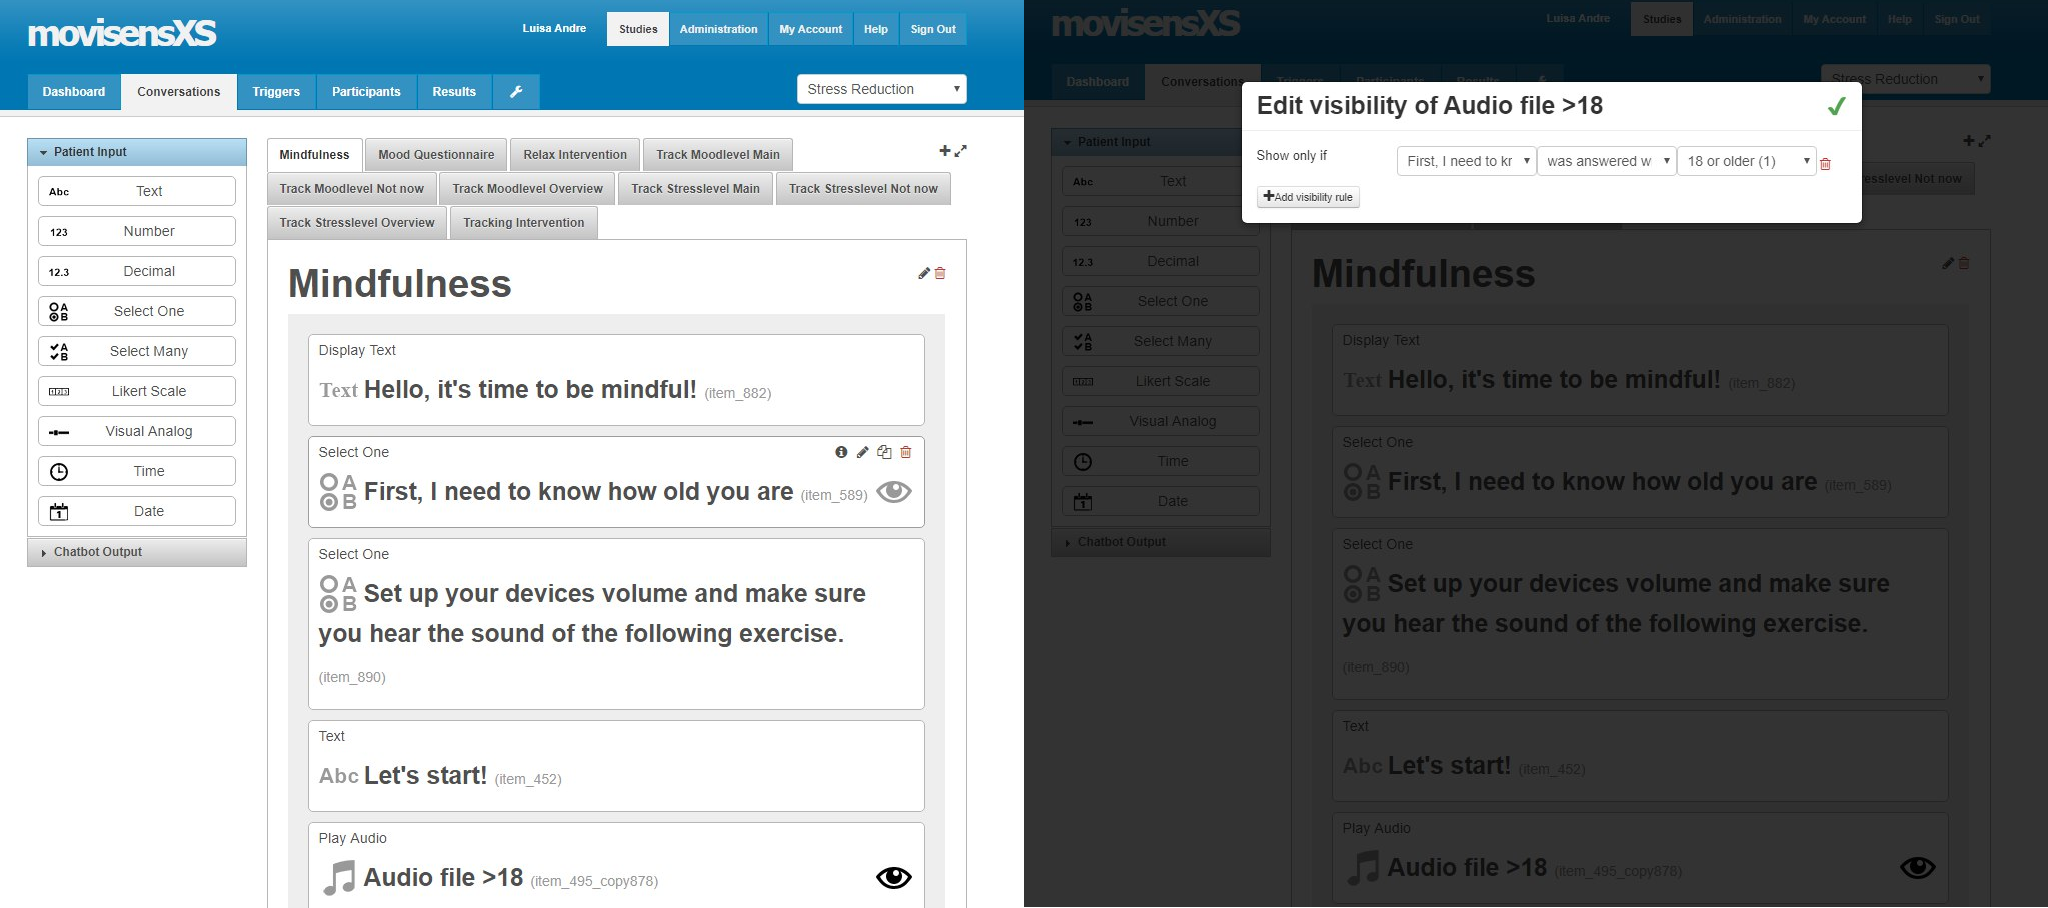
\includegraphics[width=1\textwidth]{pictures/movconv}
\caption{Die Übersicht der Konversationen des Therapie-Moduls \emph{Stress Reduction}. Links befindet sich die Werkzeugpalette mit den entsprechenden Nachrichtenformaten. Diese können per Drag and Drop sequentiell angeordnet werden. Das Auge symbolisiert eine hinterlegte Sichtbarkeitsregel. Ein Klick auf das Auge offenbart die Regel. Diese ist hier rechts zu sehen.}
\label{movconv}
\end{figure}
